\documentclass{article}
\usepackage[T1]{fontenc}
\usepackage{lmodern}
\usepackage{graphicx}
\usepackage{amsmath,amssymb}
\usepackage[a4paper,margin=2cm]{geometry}
\usepackage[absolute,overlay]{textpos}
\setlength{\TPHorizModule}{1mm}
\setlength{\TPVertModule}{1mm}
\usepackage[indonesian]{babel}
\usepackage{hyperref}
\setlength{\emergencystretch}{2em}
% unit: Halaman 18

\begin{document}

% === Halaman 18 (llm) ===

\section*{Penjelasan Analitik $P + P = 2P = R$}

Persamaan tangen $g$: $y = mx + c$

\vspace{157.41mm}

Gradien garis $g$: \[ m = \frac{dy}{dx} = \frac{3x_p^2 + a}{2y_p} \]

Perpotongan garis $g$ dengan kurva: $(mx + c)^2 = x^3 + ax + b$

Koordinat Titik R:
\begin{align*}
x_r &= m^2 - 2x_p \\
y_r &= m(x_p - x_r) - y_p
\end{align*}

Jika $y_p = 0$ maka $m$ tidak terdefinisi sehingga $2P = O$

\vspace{10mm}

Sumber gambar: Andreas Steffen, Elliptic Curve Cryptography

% deskripsi: Grafik kurva eliptik yang menunjukkan titik P, titik R, dan garis singgung g yang memotong kurva di titik P dan R, serta proyeksi titik -R
% bbox normalisasi: [0.5200, 0.2200, 0.8500, 0.7500]
\begin{textblock*}{69.30mm}(109.20mm,65.34mm)
\noindent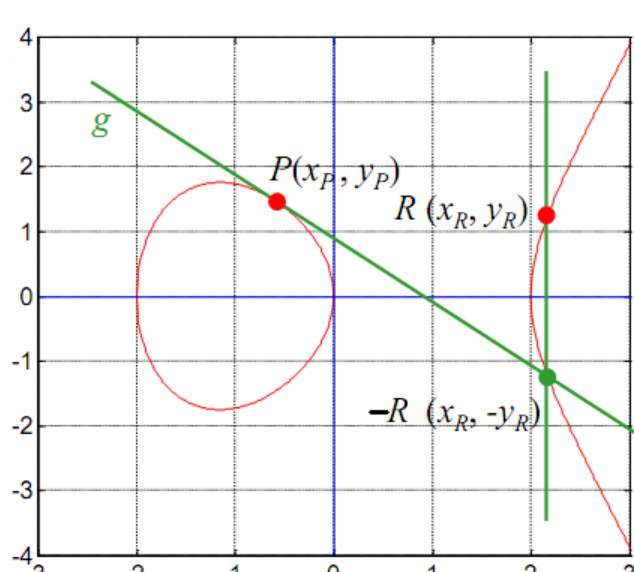
\includegraphics[width=69.30mm,height=157.41mm]{../../images/llm/page_018_img_01.png}%
\end{textblock*}

\end{document}
